\documentclass[a4paper]{article}

\usepackage[utf8]{inputenc}
\usepackage{amsmath}
\usepackage{amsfonts}
\usepackage{amssymb}
\usepackage{amsthm}
\usepackage[czech]{babel}
\usepackage{fontenc}
\usepackage{bbm}
%\usepackage[dvips,pdftex,draft]{graphicx}
\usepackage{fancyhdr} %zahlavi a zapati
\usepackage{a4wide} % širší stránka
\usepackage{todonotes}
\presetkeys{todonotes}{inline}{}
\usepackage{graphicx}
\usepackage{float}
\usepackage{hyperref}
\usepackage[
    left   = 1.0 in,
    right  = 1.0 in,
    top    = 1.5 in,
    bottom = 1.0 in,
]{geometry}

%\usepackage[dvips,pdftex]{hyperref}

\author{David Napravnik}

\begin{document}

% záhlaví vlevo
  \lhead{3. DÚ -- Splay trees}
% záhlaví uprostřed
  \chead{Datové Struktury I}
% záhlaví vpravo -- jméno
  \rhead{David Napravnik}
% nastavíme použití toho stylu
  \pagestyle{fancy}

	Počítač: Procesor AMD Ryzen 7 5800HS @ 3.20GHz, RAM 16GB.
	
	Operační systém: Windows 10, Version 10.0.19044 Build 19044
	
	Verze pythonu: 3.8.10

    Seed: 94

	\section{Abstrakt}
	Představení a porovnání dvou implementací transponování matice.
	Měří se počet netrefení se do cache a to pro obě implementace a to pro tyto velikosti cache:
	\begin{itemize}
		\item 4 kb (bloky po 16 položkách)
		\item 32 kb (bloky po 64 položkách)
		\item 256 kb (bloky po 256 položkách)	
		\item 256 kb (bloky po 4096 položkách)	
	\end{itemize}
	Implementace máme:
	\begin{itemize}
		\item naivní
		\item chache friendly
	\end{itemize}
	
	\section{Testované implementace}

	\subsection{Standardní naivní implementace}

	První implementace ignoruje cache a šahá do paměti bez rozmýšlení.

	\subsection{Chytrá cache friendly implementace}

	Druhá implementace přistupuje do paměti tak, aby co nejefektivněji využila cache.
	

	\section{Měření času}

  	Všechna měření probíhala na stejném zařízení.

	Naivní implementace běžela 3 minuty a 1 sekund (na 16ti vláknech). 

	Chytrá implementace běžela 2 minuty a 58 sekund (na 16ti vláknech). 

	Takže je jasně vidět, že python jakožto programovací jazyk je pomalý sám o sobě.
	
	\subsection{Shrnutí}

	Podle analýzi přístupů do paměti jsme zjistili, že chytrá implementace o dost
	lépe využíva cache, bohužel, to na času běhu programu, nebylo vůbec poznat.

    \begin{figure}[H]
		\centering
		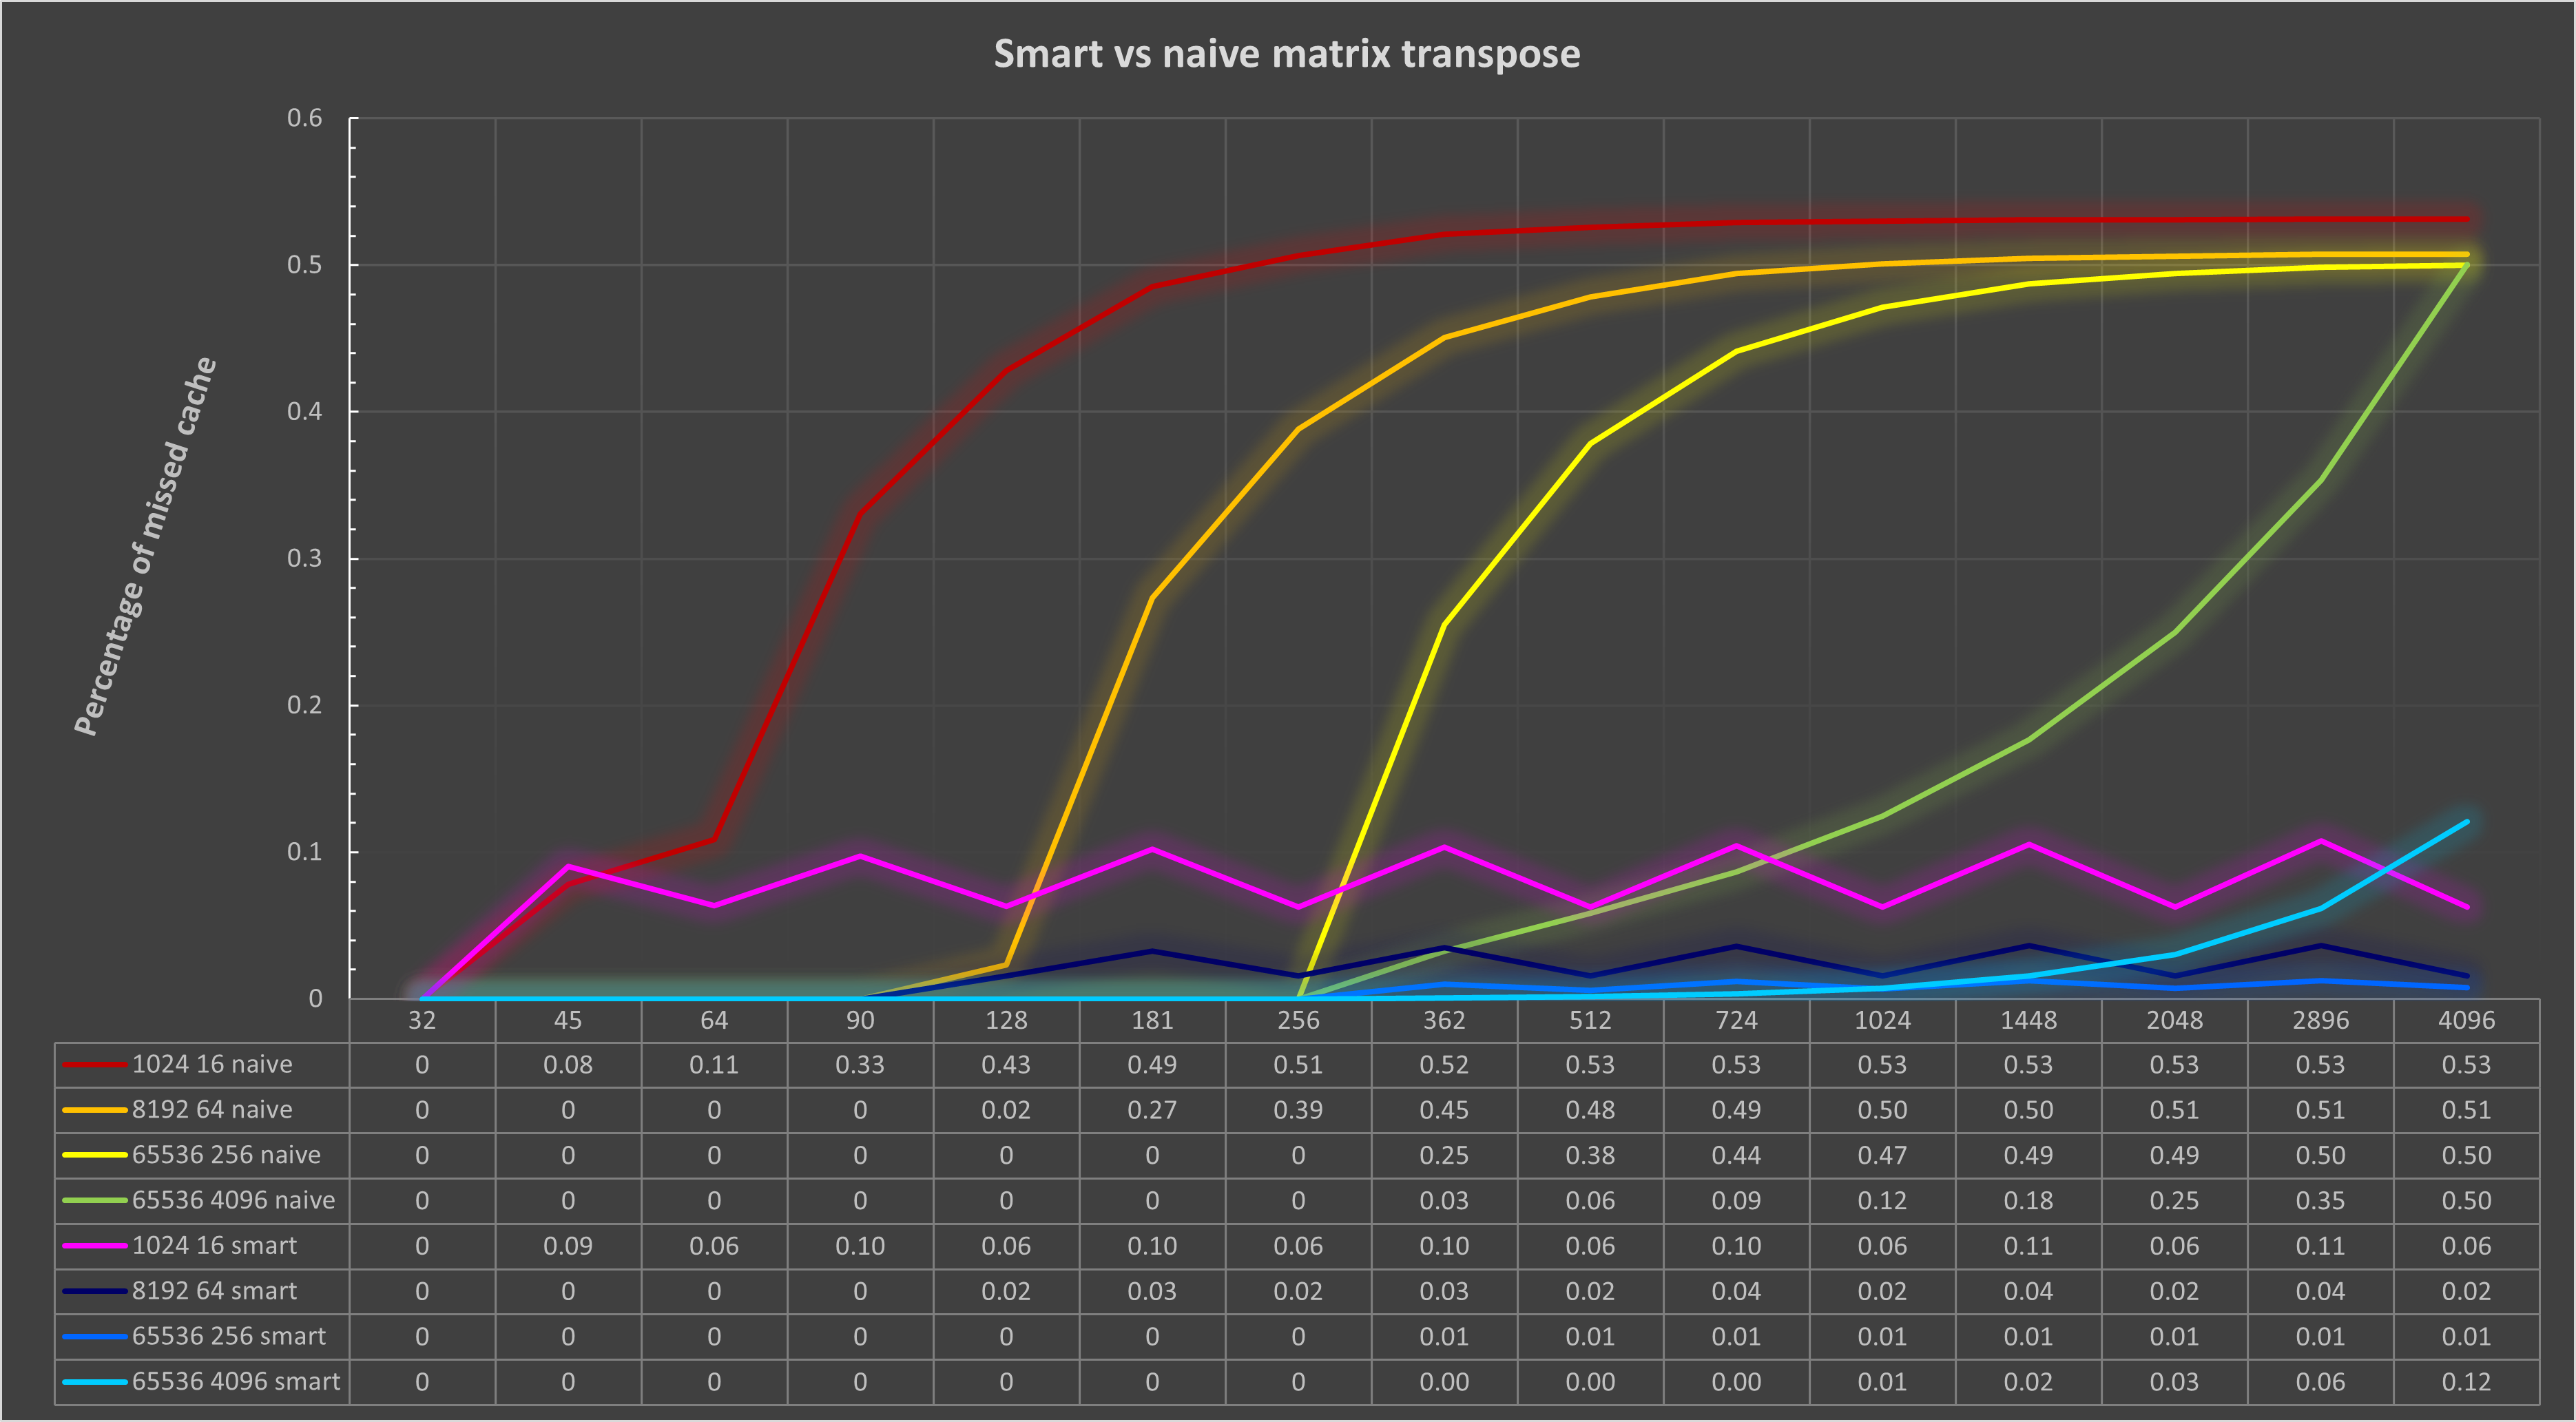
\includegraphics[angle=90,width=\textwidth,height=\textheight,keepaspectratio]{img/graph1.png}
		\caption{Porovnání dvou implementací s různou velikostí cache.}
		\label{fig:1_graph}
	\end{figure}

\end{document}
